% Options for packages loaded elsewhere
\PassOptionsToPackage{unicode}{hyperref}
\PassOptionsToPackage{hyphens}{url}
\PassOptionsToPackage{dvipsnames,svgnames,x11names}{xcolor}
%
\documentclass[
  10pt,
]{article}
\usepackage{amsmath,amssymb}
\usepackage{iftex}
\ifPDFTeX
  \usepackage[T1]{fontenc}
  \usepackage[utf8]{inputenc}
  \usepackage{textcomp} % provide euro and other symbols
\else % if luatex or xetex
  \usepackage{unicode-math} % this also loads fontspec
  \defaultfontfeatures{Scale=MatchLowercase}
  \defaultfontfeatures[\rmfamily]{Ligatures=TeX,Scale=1}
\fi
\usepackage{lmodern}
\ifPDFTeX\else
  % xetex/luatex font selection
\fi
% Use upquote if available, for straight quotes in verbatim environments
\IfFileExists{upquote.sty}{\usepackage{upquote}}{}
\IfFileExists{microtype.sty}{% use microtype if available
  \usepackage[]{microtype}
  \UseMicrotypeSet[protrusion]{basicmath} % disable protrusion for tt fonts
}{}
\makeatletter
\@ifundefined{KOMAClassName}{% if non-KOMA class
  \IfFileExists{parskip.sty}{%
    \usepackage{parskip}
  }{% else
    \setlength{\parindent}{0pt}
    \setlength{\parskip}{6pt plus 2pt minus 1pt}}
}{% if KOMA class
  \KOMAoptions{parskip=half}}
\makeatother
\usepackage{xcolor}
\usepackage[top=0.82in, bottom=0.82in, left=0.82in, right=0.82in]{geometry}
\usepackage{longtable,booktabs,array}
\usepackage{calc} % for calculating minipage widths
% Correct order of tables after \paragraph or \subparagraph
\usepackage{etoolbox}
\makeatletter
\patchcmd\longtable{\par}{\if@noskipsec\mbox{}\fi\par}{}{}
\makeatother
% Allow footnotes in longtable head/foot
\IfFileExists{footnotehyper.sty}{\usepackage{footnotehyper}}{\usepackage{footnote}}
\makesavenoteenv{longtable}
\usepackage{graphicx}
\makeatletter
\newsavebox\pandoc@box
\newcommand*\pandocbounded[1]{% scales image to fit in text height/width
  \sbox\pandoc@box{#1}%
  \Gscale@div\@tempa{\textheight}{\dimexpr\ht\pandoc@box+\dp\pandoc@box\relax}%
  \Gscale@div\@tempb{\linewidth}{\wd\pandoc@box}%
  \ifdim\@tempb\p@<\@tempa\p@\let\@tempa\@tempb\fi% select the smaller of both
  \ifdim\@tempa\p@<\p@\scalebox{\@tempa}{\usebox\pandoc@box}%
  \else\usebox{\pandoc@box}%
  \fi%
}
% Set default figure placement to htbp
\def\fps@figure{htbp}
\makeatother
\setlength{\emergencystretch}{3em} % prevent overfull lines
\providecommand{\tightlist}{%
  \setlength{\itemsep}{0pt}\setlength{\parskip}{0pt}}
\setcounter{secnumdepth}{5}
% definitions for citeproc citations
\NewDocumentCommand\citeproctext{}{}
\NewDocumentCommand\citeproc{mm}{%
  \begingroup\def\citeproctext{#2}\cite{#1}\endgroup}
\makeatletter
 % allow citations to break across lines
 \let\@cite@ofmt\@firstofone
 % avoid brackets around text for \cite:
 \def\@biblabel#1{}
 \def\@cite#1#2{{#1\if@tempswa , #2\fi}}
\makeatother
\newlength{\cslhangindent}
\setlength{\cslhangindent}{1.5em}
\newlength{\csllabelwidth}
\setlength{\csllabelwidth}{3em}
\newenvironment{CSLReferences}[2] % #1 hanging-indent, #2 entry-spacing
 {\begin{list}{}{%
  \setlength{\itemindent}{0pt}
  \setlength{\leftmargin}{0pt}
  \setlength{\parsep}{0pt}
  % turn on hanging indent if param 1 is 1
  \ifodd #1
   \setlength{\leftmargin}{\cslhangindent}
   \setlength{\itemindent}{-1\cslhangindent}
  \fi
  % set entry spacing
  \setlength{\itemsep}{#2\baselineskip}}}
 {\end{list}}
\usepackage{calc}
\newcommand{\CSLBlock}[1]{\hfill\break\parbox[t]{\linewidth}{\strut\ignorespaces#1\strut}}
\newcommand{\CSLLeftMargin}[1]{\parbox[t]{\csllabelwidth}{\strut#1\strut}}
\newcommand{\CSLRightInline}[1]{\parbox[t]{\linewidth - \csllabelwidth}{\strut#1\strut}}
\newcommand{\CSLIndent}[1]{\hspace{\cslhangindent}#1}
\usepackage{xcolor}
\usepackage{hyperref}
\hypersetup{colorlinks=true, linkcolor=blue, urlcolor=blue, citecolor=blue}
\usepackage{float}
\usepackage{booktabs}
\usepackage{caption}
\usepackage{enumitem}
\usepackage{fancyhdr}
\usepackage{lastpage}
\usepackage{microtype}
\usepackage{titlesec}
\usepackage{setspace}
\usepackage{fvextra}
\setcounter{secnumdepth}{0}
\floatplacement{figure}{H}
\floatplacement{table}{H}
\captionsetup{font=footnotesize, labelfont=bf}
\setlength{\parindent}{0pt}
\setlength{\parskip}{0.18em}
\setlist{nosep,leftmargin=*}
\titlespacing*{\section}{0pt}{0.44em}{0.15em}
\titlespacing*{\subsection}{0pt}{0.34em}{0.12em}
\titleformat{\section}{\large\bfseries}{\thesection}{0.5em}{}
\titleformat{\subsection}{\normalsize\bfseries}{\thesubsection}{0.5em}{}
\makeatletter
\renewcommand{\maketitle}{}
\makeatother
\AtBeginEnvironment{figure}{\singlespacing}
\AtBeginEnvironment{table}{\singlespacing}
\fancypagestyle{plain}{
  \fancyhf{}
  \renewcommand{\headrulewidth}{0pt}
  \renewcommand{\footrulewidth}{0pt}
  \fancyfoot[C]{\small Page~\thepage~of~\pageref{LastPage}}
}
\pagestyle{fancy}
\fancyhf{}
\setlength{\headheight}{13pt}
\fancyhead[L]{\small Saijo}
\fancyhead[R]{\small GSAx Time Series}
\fancyfoot[C]{\small Page~\thepage~of~\pageref{LastPage}}
\renewcommand{\headrulewidth}{0.35pt}
\renewcommand{\footrulewidth}{0.35pt}
\sloppy
\usepackage{booktabs}
\usepackage{longtable}
\usepackage{array}
\usepackage{multirow}
\usepackage{wrapfig}
\usepackage{float}
\usepackage{colortbl}
\usepackage{pdflscape}
\usepackage{tabu}
\usepackage{threeparttable}
\usepackage{threeparttablex}
\usepackage[normalem]{ulem}
\usepackage{makecell}
\usepackage{xcolor}
\usepackage{bookmark}
\IfFileExists{xurl.sty}{\usepackage{xurl}}{} % add URL line breaks if available
\urlstyle{same}
\hypersetup{
  pdftitle={Are Goals Saved Above Expected Team-Independent?},
  pdfauthor={Rento Saijo},
  colorlinks=true,
  linkcolor={blue},
  filecolor={Maroon},
  citecolor={blue},
  urlcolor={blue},
  pdfcreator={LaTeX via pandoc}}

\title{Are Goals Saved Above Expected Team-Independent?}
\usepackage{etoolbox}
\makeatletter
\providecommand{\subtitle}[1]{% add subtitle to \maketitle
  \apptocmd{\@title}{\par {\large #1 \par}}{}{}
}
\makeatother
\subtitle{A Game-by-Game Time Series Study of Mackenzie Blackwood and Igor Shesterkin}
\author{Rento Saijo}
\date{May 12, 2026}

\begin{document}
\maketitle

\begin{titlepage}
\thispagestyle{empty}
\begin{center}
\vspace*{\fill}
{\LARGE\bfseries Are Goals Saved Above Expected Team-Independent?\par}
\vspace{0.22in}
{\large A Game-by-Game Time Series Study of Mackenzie Blackwood and Igor Shesterkin\par}
\vspace{0.35in}
{\normalsize Rento Saijo\par}
\vspace{0.14in}
{\normalsize STA 209: Introduction to Time Series Analysis\par}
{\normalsize Professor Priya Kohli\par}
\vspace{0.14in}
{\normalsize May 12, 2026\par}
\vspace*{\fill}
\end{center}
\end{titlepage}
\setcounter{page}{1}
\doublespacing

\section{Abstract}\label{abstract}

Goals saved above expected, or GSAx, is used in hockey because it tries to judge a goalie after accounting for shot quality. That promise raises a time-series question: once chance quality and recent goalie performance are considered, is there still meaningful game-to-game structure in a goalie's GSAx, and does that structure look different for a goalie who changed teams? I study 285 matched regular-season even-strength games for Mackenzie Blackwood and Igor Shesterkin. Blackwood's path moves through New Jersey, San Jose, and Colorado, while Shesterkin remains with the Rangers, so the comparison contrasts changing team context with organizational continuity. The response is game-by-game even-strength GSAx; the predictors are game-level even-strength save percentage and team even-strength xGF\%. All six raw series are stationary by ADF tests, no convincing game-index seasonality appears, and the final transformed lagged regressions explain little of the game-to-game variation. Shesterkin's lagged predictors are jointly significant but small in explanatory power, while Blackwood's are not jointly significant. ARMA and ARIMA checks select white-noise residual models for both goalies, so the final model explains the remaining dependence mainly by showing how little stable dependence is left.

\section{Introduction}\label{introduction}

Hockey goaltending is hard to evaluate because the goalie is visible at the end of every failed defensive sequence. A raw goal against may come from a clean shot that should be stopped, but it may also come from a backdoor pass, a screen, a rebound, or a rush chance that puts the goalie in a much harder position. This is why expected-goals models matter. They estimate shot danger before the result is known, and GSAx compares the goals a goalie actually allows to the goals an expected-goals model would have expected from those chances. Positive GSAx means the goalie stopped more than expected; negative GSAx means the opposite. Prior work supports this framing because scoring chances are shaped by tactical and contextual variables (\citeproc{ref-lignell2020}{Lignell, Rago, and Mohr 2020}), and expected-goals-type process measures can improve performance evaluation beyond raw shot or goal counts (\citeproc{ref-mead2023}{Mead, O'Hare, and McMenemy 2023}). Goalkeeper-specific expected-goals work also makes the conceptual point that keeper performance and chance quality need to be separated carefully rather than blended into one outcome (\citeproc{ref-delacruz2025}{De-la-Cruz-Torres, Navarro-Castro, and Ruiz-de-Alarcón-Quintero 2025}).

The research question is whether lagged goalie performance and lagged team shot-quality context explain current game-by-game even-strength GSAx after removing simple average levels. I use Blackwood and Shesterkin because the comparison is useful without requiring the reader to know NHL team histories. Blackwood changed team environments substantially, while Shesterkin stayed in one organization during the matched sample. If GSAx were perfectly team-independent and essentially unpredictable from recent team context, lagged team xGF\% should not add much. If goalie form carried clear short-run momentum, lagged save percentage should add stronger predictive structure. The hypothesis is therefore conservative: lagged save percentage may contain some short-run information, lagged team xGF\% may matter weakly, but after stationarity, transformation, and regression, the remaining residuals should be close to white noise.

\section{Methodology}\label{methodology}

The unit of observation is one completed regular-season game at even strength. Let \(G_t\) be game-by-game even-strength GSAx in goals, \(S_t\) be even-strength save percentage as a proportion, and \(X_t\) be team even-strength xGF\% in percentage points. I first plot all series and use the Augmented Dickey-Fuller test, whose null hypothesis is non-stationarity. Since the game index is not a calendar month or quarter, I use periodograms only to check whether the response or predictors contain a credible repeating game-cycle frequency. The periodograms did not show stable, interpretable seasonality, so the trend model is the constant mean model \(Y_t=\mu_Y+W_t\), and detrending means subtracting the fitted average level.

The time-series regression uses only lagged predictors, because same-game or future predictor information would not be available for forecasting. Cross-correlation functions suggested \(\tilde{S}_{t-4}\) and \(\tilde{X}_{t-8}\) for Blackwood and \(\tilde{S}_{t-2}\) and \(\tilde{X}_{t-4}\) for Shesterkin, where tildes mean deviations from each goalie's fitted average; the supporting CCF evidence is shown in Figure \ref{fig:ccf-plot} and Table \ref{tab:ccf-table} from Appendix A, with the corresponding lagged scatterplots in Figures \ref{fig:scatter-blackwood-sv}-\ref{fig:scatter-shesterkin-xgf} from Appendix A. The response needed a shifted Box-Cox transformation to reduce variance imbalance, summarized in Table \ref{tab:transform-table} from Appendix A, so the fitted regression is \(Y_t=\beta_0+\beta_1\tilde{S}_{t-a}+\beta_2\tilde{X}_{t-b}+W_t\) on the transformed detrended-GSAx scale. Finally, I inspect the residual plots, ACF, and PACF and compare low-order ARMA and first-differenced ARIMA candidates by AIC. As a benchmark, I also let \texttt{forecast::auto.arima()} choose an ARIMA error structure with \(S_t\) and \(X_t\) included as external regressors.

\section{Results and Conclusion}\label{results-and-conclusion}

\begin{table}[H]
\centering
\caption{\label{tab:sample-summary}Matched game-by-game even-strength samples.}
\centering
\resizebox{\ifdim\width>\linewidth\linewidth\else\width\fi}{!}{
\fontsize{6.6}{8.6}\selectfont
\begin{tabular}[t]{lccrrrr}
\toprule
Goalie & Teams & Dates & Games & Mean GSAx & Mean SV\% & Mean xGF\%\\
\midrule
Mackenzie Blackwood & NJD, SJS, COL & 2018-12-18 to 2026-03-28 & 285 & -0.040 & 0.902 & 48.59\\
Igor Shesterkin & NYR & 2020-01-07 to 2025-11-04 & 285 & 0.233 & 0.916 & 49.07\\
\bottomrule
\end{tabular}}
\end{table}

Table \ref{tab:sample-summary} gives the final sample. The plots in Figure \ref{fig:main-series} show why the final paper uses game-by-game GSAx rather than cumulative GSAx. The game-level response fluctuates around a stable center for both goalies, while Blackwood's team context visibly changes around the vertical franchise-change markers. All six ADF tests reject non-stationarity at the 5\% level (Table \ref{tab:stationarity-table} from Appendix A), and the periodogram evidence does not justify harmonic seasonal terms (Figure \ref{fig:periodogram-plot} and Table \ref{tab:periodogram-table} from Appendix A). In hockey terms, this is plausible: a game number is a repeated performance index, not a calendar season with a fixed monthly rhythm.

\begin{figure}[H]

{\centering 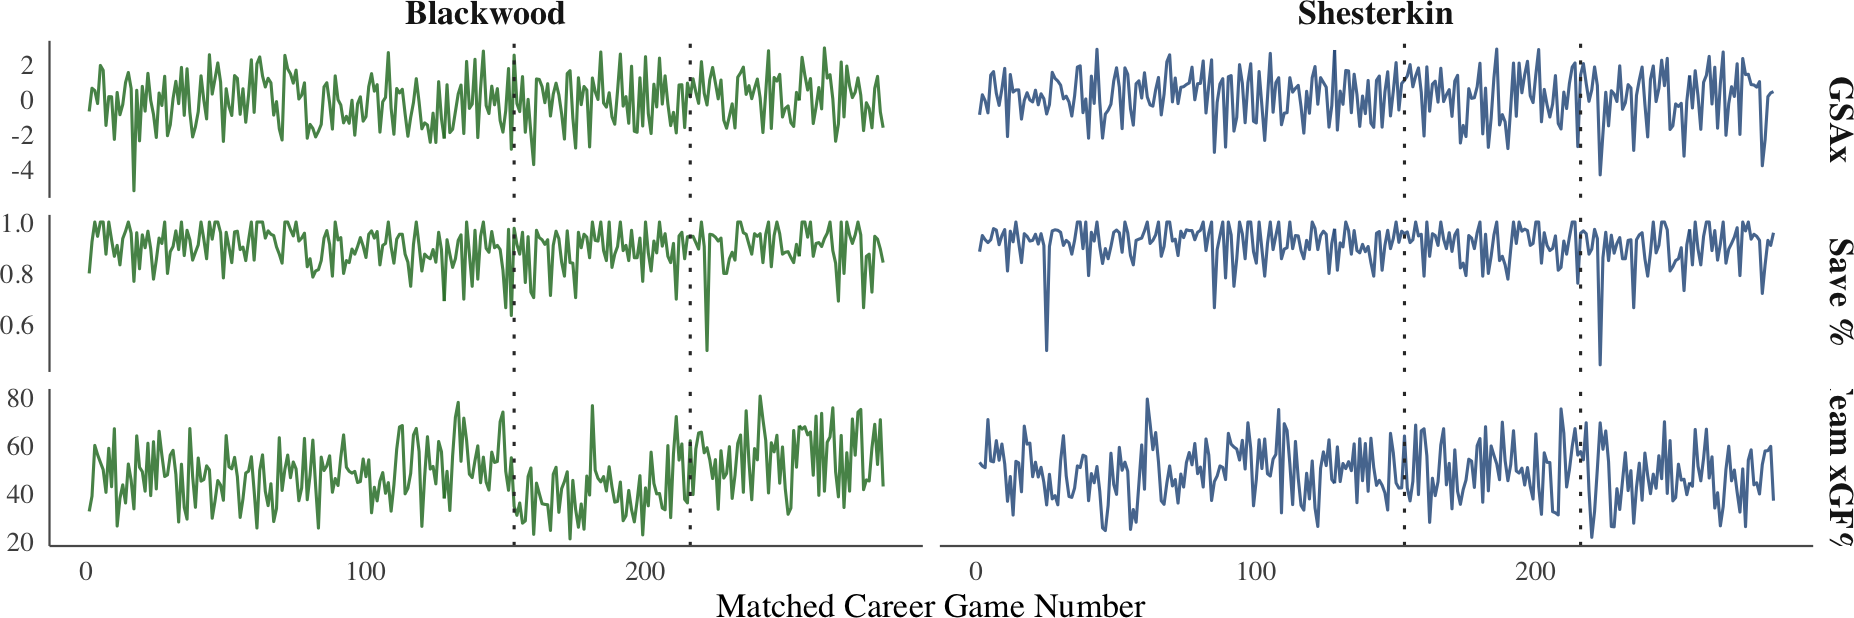
\includegraphics[width=\linewidth]{Paper_files/figure-latex/main-series-1} 

}

\caption{Game-by-game even-strength response and predictors. Dotted vertical lines mark Blackwood franchise changes; Shesterkin stayed with the Rangers in the matched sample.}\label{fig:main-series}
\end{figure}

\begin{table}[H]
\centering
\caption{\label{tab:model-comparison}Final model comparison. Manual residual AIC is on the transformed residual scale; auto.arima uses raw GSAx with raw save percentage and team xGF\% as xreg.}
\centering
\resizebox{\ifdim\width>\linewidth\linewidth\else\width\fi}{!}{
\fontsize{6.2}{8.2}\selectfont
\begin{tabular}[t]{l>{\raggedright\arraybackslash}p{1.25in}>{\raggedright\arraybackslash}p{1.25in}>{\raggedright\arraybackslash}p{1.25in}>{\raggedright\arraybackslash}p{1.2in}}
\toprule
Goalie & TS Regression & Manual Residual Model & Best Differenced Candidate & auto.arima + xreg\\
\midrule
Blackwood & $R_a^2=0.0083$; $p_F=0.1182$ & ARIMA(0,0,0); AIC 1630.45 & ARIMA(0,1,1); AIC 1632 & ARIMA(0,1,1); AIC 706.58\\
Shesterkin & $R_a^2=0.0324$; $p_F=0.0038$ & ARIMA(0,0,0); AIC 1889.83 & ARIMA(0,1,1); AIC 1891.75 & ARIMA(0,1,1); AIC 598.03\\
\bottomrule
\end{tabular}}
\end{table}

The regression evidence in Table \ref{tab:model-comparison}, with coefficient, fit, and forecast-evaluation details in Tables \ref{tab:coef-tables}-\ref{tab:forecast-eval-table} from Appendix B, answers the main question with a useful null result. For Blackwood, the lagged transformed regression has adjusted \(R^2=0.0083\) and \(p_F=0.1182\), so I do not have evidence that lagged save percentage and team xGF\% jointly explain current transformed detrended GSAx. For Shesterkin, the same test is statistically significant with adjusted \(R^2=0.0324\) and \(p_F=0.0038\), but the explanatory power is still small. In words, Shesterkin has a detectable short-run lagged relationship, mostly around the two-game save-percentage lead, yet most of his game-to-game GSAx remains unexplained by these two lagged variables. Blackwood's changing team environment is visible descriptively, but in this regression design it does not become a strong predictor of next-game transformed GSAx. The final fitted models on the original GSAx scale are, for Blackwood,
\[
\begin{aligned}
G_t = -0.0400
&+ \left[1.6711\left\{12.1729 - 5.5234(S_{t-4}-0.9023)\right.\right.\\
&\left.\left.- 0.0321(X_{t-8}-48.5914) + W_t\right\} + 1\right]^{1/1.6711}
- 6.1500,
\end{aligned}
\]
and, for Shesterkin,
\[
\begin{aligned}
G_t = 0.2329
&+ \left[1.9999\left\{15.7009 - 17.0007(S_{t-2}-0.9163)\right.\right.\\
&\left.\left.+ 0.0542(X_{t-4}-49.0655) + W_t\right\} + 1\right]^{1/1.9999}
- 5.5209.
\end{aligned}
\]
These equations show the model sequence directly: subtract the fitted average levels, transform the detrended response, fit the lagged regression, and then reverse the response transformation so fitted values are again measured in goals.

\begin{figure}[H]

{\centering 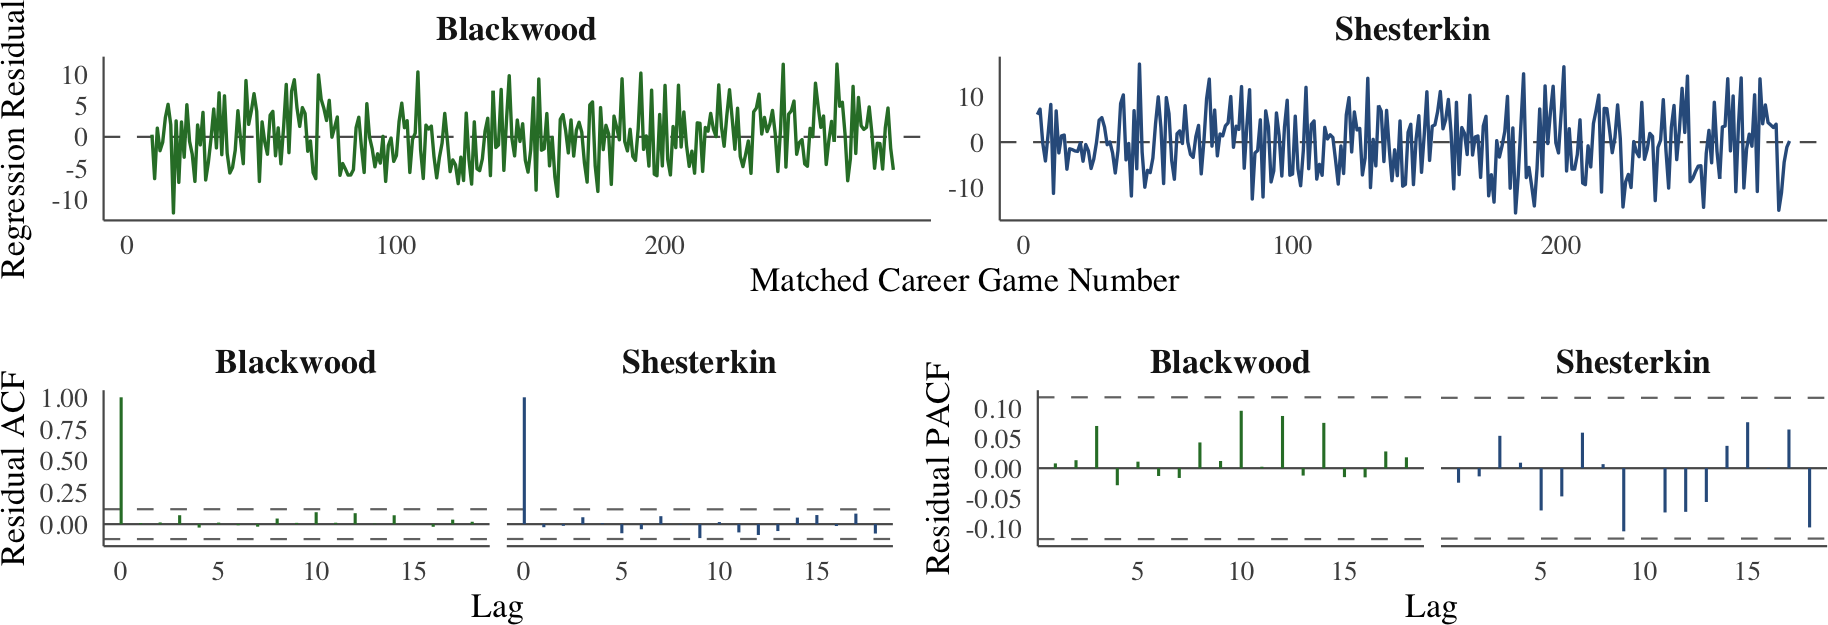
\includegraphics[width=\linewidth]{Paper_files/figure-latex/residual-diagnostics-1} 

}

\caption{Residual index plots, residual ACF, and residual PACF after the transformed lagged regressions.}\label{fig:residual-diagnostics}
\end{figure}

Figure \ref{fig:residual-diagnostics} shows why the residual model remains simple. The residuals fluctuate around zero without a sustained trend or visible seasonal cycle, and the ACF and PACF spikes do not form a slow-decaying dependence pattern. The broader original-transformed-residual comparison in Figure \ref{fig:acf-pacf-comparison} from Appendix C tells the same story: any small serial structure before modeling is not strong enough to survive as useful residual dependence. The low-order ARMA comparison selects ARMA(0,0), written here as ARIMA(0,0,0), for both goalies (Tables \ref{tab:arma-candidates-blackwood} and \ref{tab:arma-candidates-shesterkin} from Appendix C). First-differenced ARIMA candidates do not improve AIC (Table \ref{tab:arima-candidate-table} from Appendix C), and I do not fit ARCH/GARCH models because the residual plots do not show clear volatility clustering or changing conditional variance. Therefore, the final fitted model is a transformed lagged regression plus white-noise residuals. With future lagged predictors set to each goalie's fitted average levels, the ten-game GSAx forecasts are essentially flat, with wide bands that reflect how noisy single-game goaltending outcomes are.

\begin{figure}[H]

{\centering 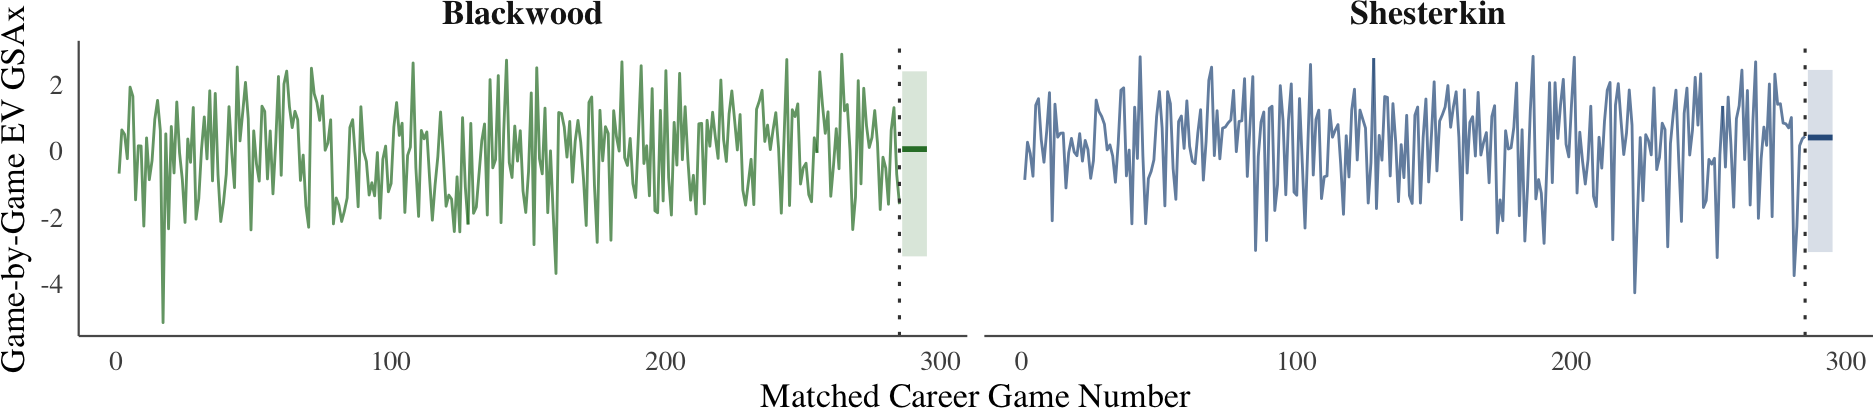
\includegraphics[width=\linewidth]{Paper_files/figure-latex/forecast-plot-1} 

}

\caption{Ten-game response forecasts from the final manual model under average future predictor conditions. The dotted line marks the last observed matched game.}\label{fig:forecast-plot}
\end{figure}

The automated benchmark in Table \ref{tab:model-comparison}, with innovation variance and information criteria in Table \ref{tab:auto-table} from Appendix C, selects ARIMA(0,1,1) errors for both goalies. Written as one regression-with-ARIMA-errors equation for each goalie, the fitted benchmarks are
\[
\begin{aligned}
\text{Blackwood:}\quad G_t &= G_{t-1}+14.3200(S_t-S_{t-1})-0.0040(X_t-X_{t-1})+W_t-0.9700W_{t-1},\\
\text{Shesterkin:}\quad G_t &= G_{t-1}+16.0185(S_t-S_{t-1})-0.0128(X_t-X_{t-1})+W_t-0.9861W_{t-1}.
\end{aligned}
\]
The automated model has lower raw-scale AIC, and the MA coefficient near \(-1\) says the fitted series mainly adjusts through one-game changes rather than persistent autoregression (as commented in homework 7). Still, it is more mechanical than the final model because it uses current changes in \(S_t\) and \(X_t\), while the manual model follows the lagged evidence available before the game and then checks whether the remaining residuals need ARMA/ARIMA structure. Therefore, \texttt{auto.arima()} is useful as a benchmark, but the final transformed lagged-regression model is the better answer to the research question because it is built around interpretable pre-game predictors and leaves residuals that look close to white noise.

In conclusion, in these matched game-by-game even-strength series, lagged team xGF\% and lagged save percentage explain little current GSAx variation, and after the final regression there is little remaining autocorrelation to model. GSAx remains valuable because it adjusts for chance quality, but single-game GSAx is still very noisy. Blackwood shows no strong regression evidence that recent team environment predicts current GSAx; Shesterkin's lagged relationship is statistically detectable but practically small.

\section{Discussion}\label{discussion}

If I continued this research, I would expand beyond two goalies and add destination-specific team features rather than relying only on lagged team xGF\%. A larger hierarchical model could separate player ability, team environment, opponent strength, schedule density, and era. I would also test rolling-window features, rest days, back-to-back games, score state, and opponent shot quality by game situation. Finally, I would move from neutral predictor forecasts to scenario forecasts.

\section{References}\label{references}

\small
\singlespacing

\phantomsection\label{refs}
\begin{CSLReferences}{1}{0}
\bibitem[\citeproctext]{ref-delacruz2025}
De-la-Cruz-Torres, B., M. Navarro-Castro, and D. Ruiz-de-Alarcón-Quintero. 2025. {``An Expected Goals on Target (xGOT) Model: Accounting for Goalkeeper Performance in Football.''} \emph{Big Data and Cognitive Computing} 9 (3): 64. \url{https://doi.org/10.3390/bdcc9030064}.

\bibitem[\citeproctext]{ref-lignell2020}
Lignell, E., V. Rago, and M. Mohr. 2020. {``Analysis of Goal Scoring Opportunities in Elite Male Ice Hockey in Relation to Tactical and Contextual Variables.''} \emph{International Journal of Performance Analysis in Sport} 20 (6): 1003--17. \url{https://doi.org/10.1080/24748668.2020.1823161}.

\bibitem[\citeproctext]{ref-mead2023}
Mead, J., A. O'Hare, and P. McMenemy. 2023. {``Expected Goals in Football: Improving Model Performance and Demonstrating Value.''} \emph{PLOS ONE} 18 (4): e0282295. \url{https://doi.org/10.1371/journal.pone.0282295}.

\bibitem[\citeproctext]{ref-rentosrink}
Saijo, Rento. 2026a. {``Rento's Rink Expected Goal Model and Game-by-Game Data Pipeline.''} \url{https://rentosrink.streamlit.app/expected_goal}.

\bibitem[\citeproctext]{ref-sta209data}
---------. 2026b. {``STA 209 Goalie Game-by-Game Project Data.''} \url{https://github.com/RentoSaijo/STA209/tree/main/data}.

\end{CSLReferences}

\section{Data Resources}\label{data-resources}

\small
\singlespacing

The final analysis files are \texttt{data/blackwood\_gbgs.csv} and \texttt{data/shesterkin\_gbgs.csv} in this STA 209 repository (\citeproc{ref-sta209data}{Saijo 2026b}), built from the \texttt{rentosrink} game-by-game pipeline and expected-goals model (\citeproc{ref-rentosrink}{Saijo 2026a}). I used the even-strength columns named above and matched both goalies to 285 regular-season games.

\normalsize
\doublespacing

\newpage
\singlespacing

\section{Appendix}\label{appendix}

\subsection{Appendix A: Stationarity, Leads, and Transformation}\label{appendix-a-stationarity-leads-and-transformation}

\begin{table}[H]
\centering
\caption{\label{tab:stationarity-table}ADF tests for response and predictor series.}
\centering
\resizebox{\ifdim\width>\linewidth\linewidth\else\width\fi}{!}{
\fontsize{7}{9}\selectfont
\begin{tabular}[t]{lcrrcc}
\toprule
Goalie & Series & DF & Lag & P-value & Decision\\
\midrule
Blackwood & $G_t$ & -6.7931 & 6 & <0.01 & Reject $H_0$\\
Blackwood & $S_t$ & -6.0001 & 6 & <0.01 & Reject $H_0$\\
Blackwood & $X_t$ & -4.1809 & 6 & <0.01 & Reject $H_0$\\
Shesterkin & $G_t$ & -6.7433 & 6 & <0.01 & Reject $H_0$\\
Shesterkin & $S_t$ & -6.9665 & 6 & <0.01 & Reject $H_0$\\
Shesterkin & $X_t$ & -6.8293 & 6 & <0.01 & Reject $H_0$\\
\bottomrule
\end{tabular}}
\end{table}

Table \ref{tab:stationarity-table} reports the formal ADF checks that support the stationarity claim in the main paper. Because every p-value is below 0.05, the tests reject the non-stationarity null for each goalie and each study variable. This means the game-by-game series behave more like fluctuations around stable average levels than like drifting level series.

\begin{figure}[H]

{\centering 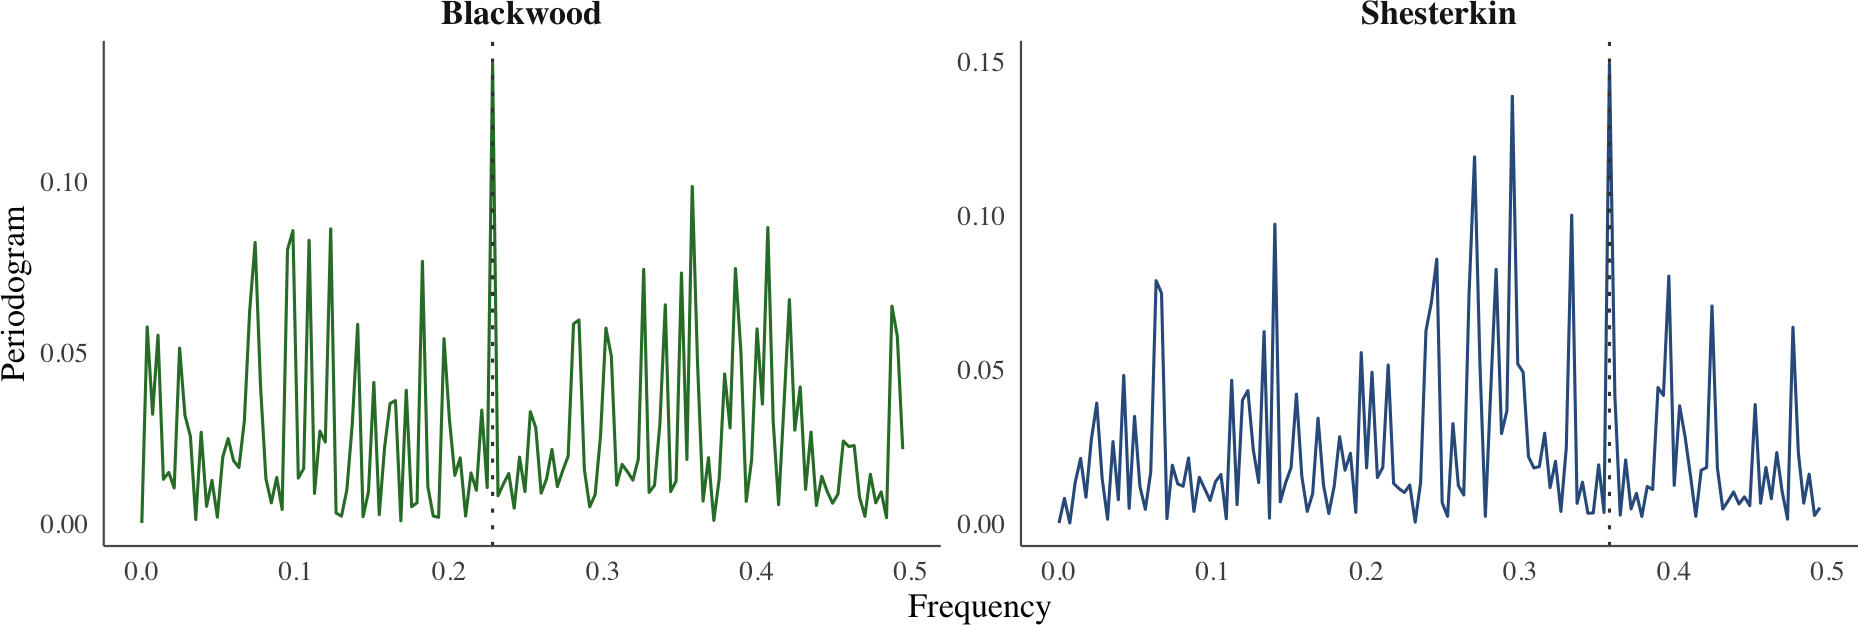
\includegraphics[width=\linewidth]{Paper_files/figure-latex/periodogram-plot-1} 

}

\caption{Response periodograms for game-by-game even-strength GSAx.}\label{fig:periodogram-plot}
\end{figure}

\begin{table}[H]
\centering
\caption{\label{tab:periodogram-table}Dominant periodogram peaks for response and predictor series.}
\centering
\resizebox{\ifdim\width>\linewidth\linewidth\else\width\fi}{!}{
\fontsize{6.8}{8.8}\selectfont
\begin{tabular}[t]{lcrr}
\toprule
Goalie & Series & Dominant Frequency & Implied Period\\
\midrule
Blackwood & $G_t$ & 0.2281 & 4.38\\
Blackwood & $S_t$ & 0.3579 & 2.79\\
Blackwood & $X_t$ & 0.0070 & 142.50\\
Shesterkin & $G_t$ & 0.3579 & 2.79\\
Shesterkin & $S_t$ & 0.3333 & 3.00\\
Shesterkin & $X_t$ & 0.0912 & 10.96\\
\bottomrule
\end{tabular}}
\end{table}

Figure \ref{fig:periodogram-plot} gives the response-variable periodograms used for the seasonality check, and Table \ref{tab:periodogram-table} gives the numerical peak summary for all three study variables. The largest peaks are sample peaks in noisy game-index data, not clean recurring cycles. Since the implied periods are not tied to a meaningful hockey calendar or a stable repeated game pattern, I do not add harmonic seasonal terms to the final models.

\begin{figure}[H]

{\centering 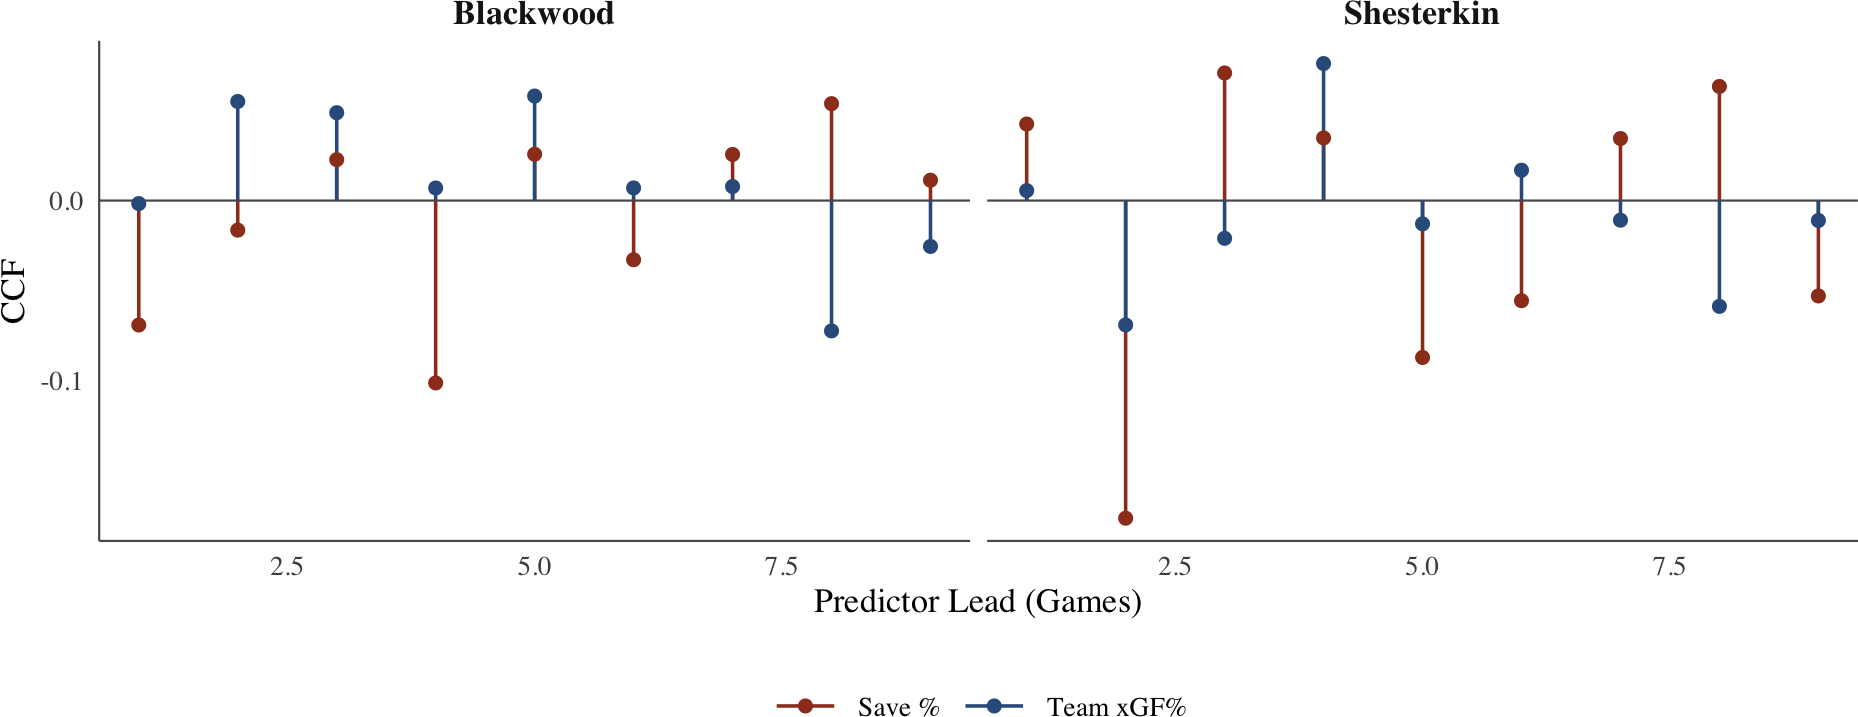
\includegraphics[width=\linewidth]{Paper_files/figure-latex/ccf-plot-1} 

}

\caption{Lead-only CCF values used to choose lagged predictors for the time-series regressions.}\label{fig:ccf-plot}
\end{figure}

\begin{table}[H]
\centering
\caption{\label{tab:ccf-table}Strongest selected predictor leads over leads 1 through 9.}
\centering
\resizebox{\ifdim\width>\linewidth\linewidth\else\width\fi}{!}{
\fontsize{7}{9}\selectfont
\begin{tabular}[t]{lcrr}
\toprule
Goalie & Predictor & Selected Lead & CCF\\
\midrule
Blackwood & $\tilde{S}$ & 4 & -0.1011\\
Blackwood & $\tilde{X}$ & 8 & -0.0723\\
Shesterkin & $\tilde{S}$ & 2 & -0.1762\\
Shesterkin & $\tilde{X}$ & 4 & 0.0760\\
\bottomrule
\end{tabular}}
\end{table}

Figure \ref{fig:ccf-plot} shows the lead-only cross-correlations used to avoid using same-game or future information. Table \ref{tab:ccf-table} records the selected leads: four games for Blackwood save percentage, eight games for Blackwood team xGF\%, two games for Shesterkin save percentage, and four games for Shesterkin team xGF\%. These CCF values are small, so the selected leads should be read as the strongest available candidates rather than strong evidence of deterministic relationships.

\begin{figure}[H]

{\centering 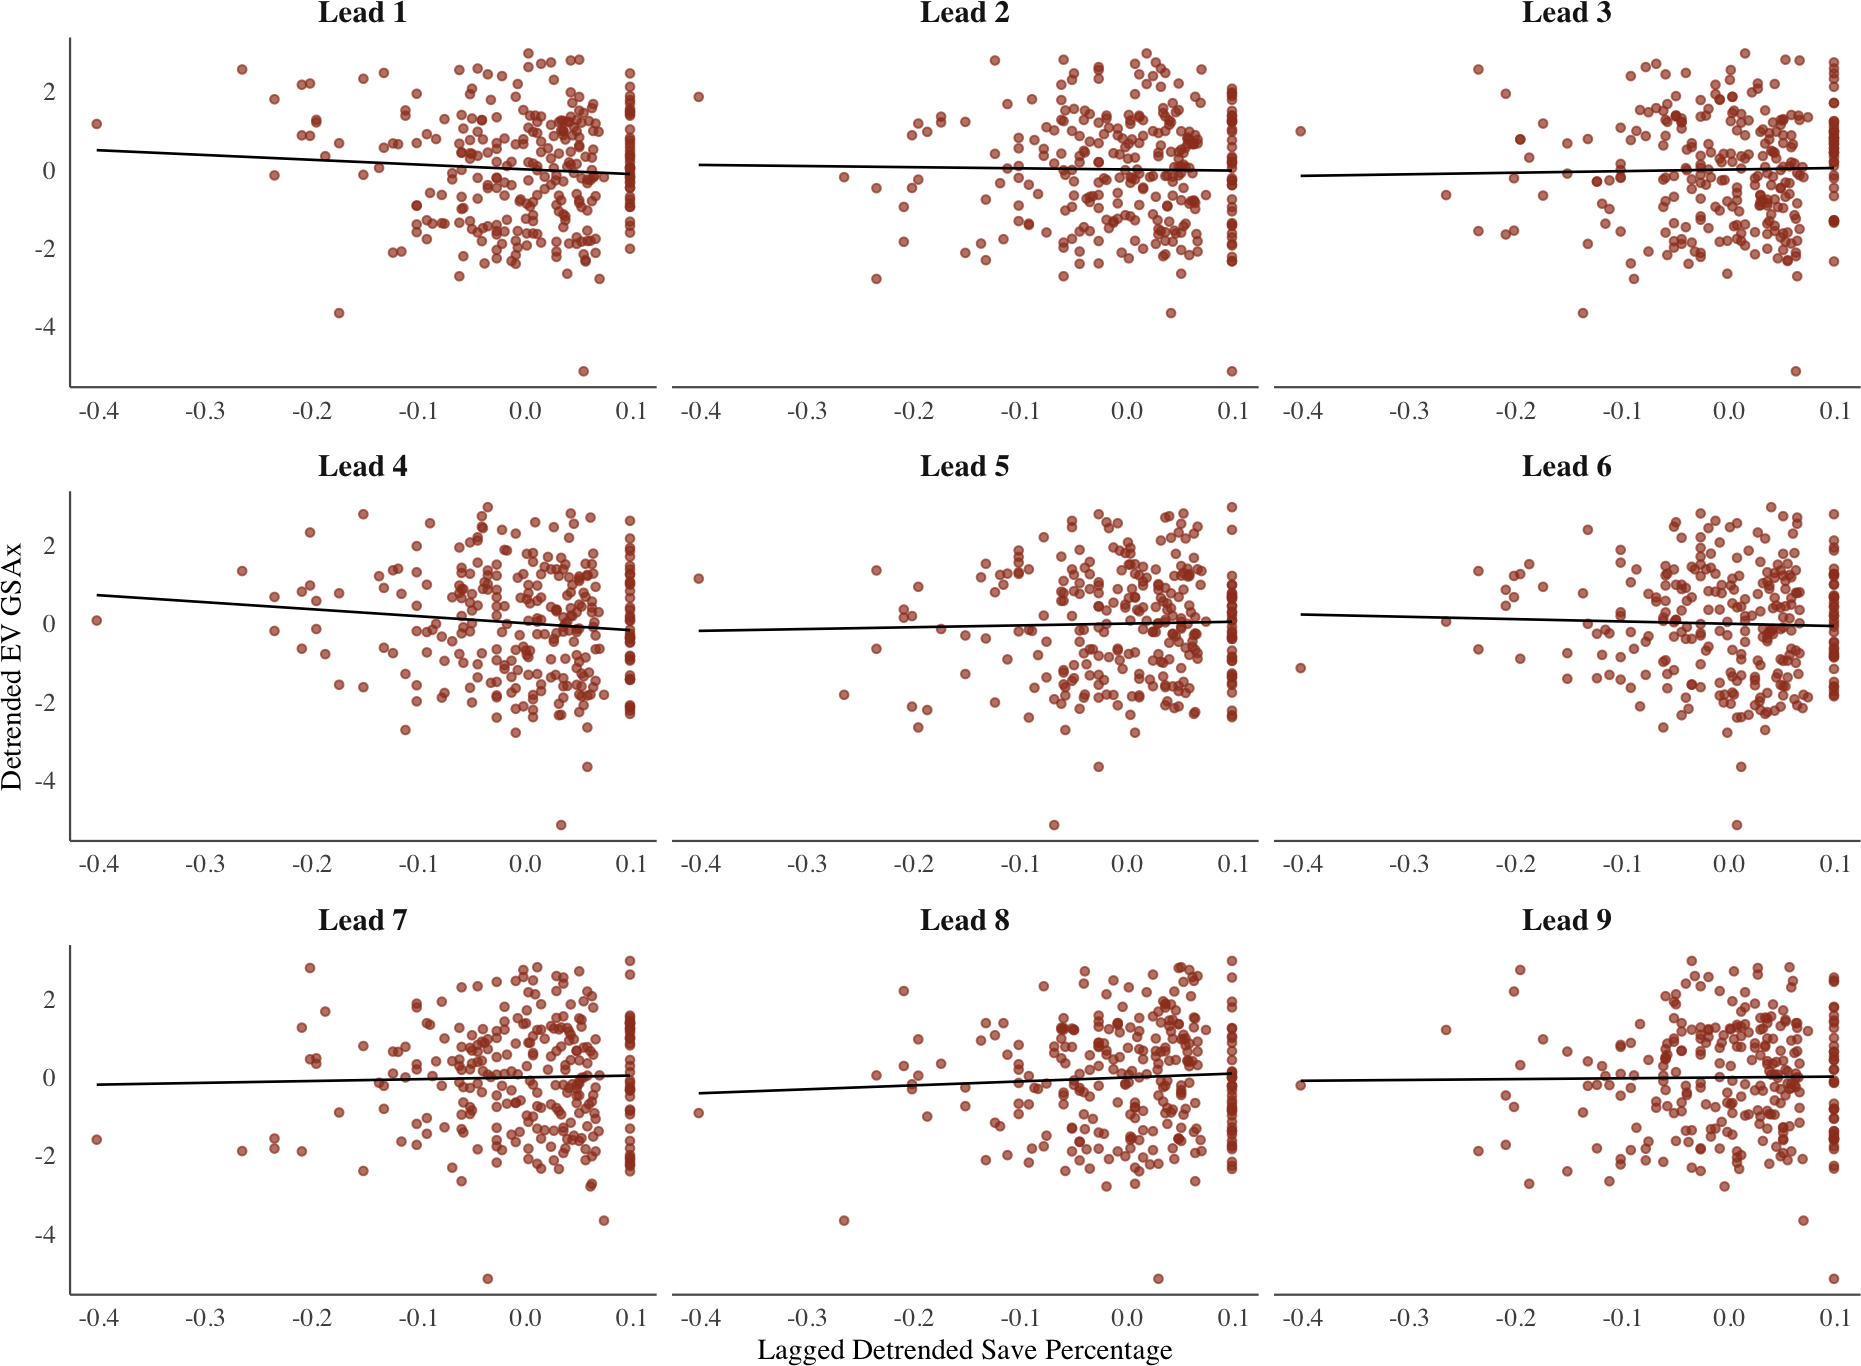
\includegraphics[width=\linewidth]{Paper_files/figure-latex/scatter-blackwood-sv-1} 

}

\caption{Blackwood detrended GSAx against lagged detrended save percentage.}\label{fig:scatter-blackwood-sv}
\end{figure}

Figure \ref{fig:scatter-blackwood-sv} shows Blackwood's detrended GSAx against lagged detrended save percentage for leads 1 through 9. The point clouds are diffuse across the panels, so the selected four-game lead should be read as the strongest available candidate rather than a strong linear relationship.

\begin{figure}[H]

{\centering 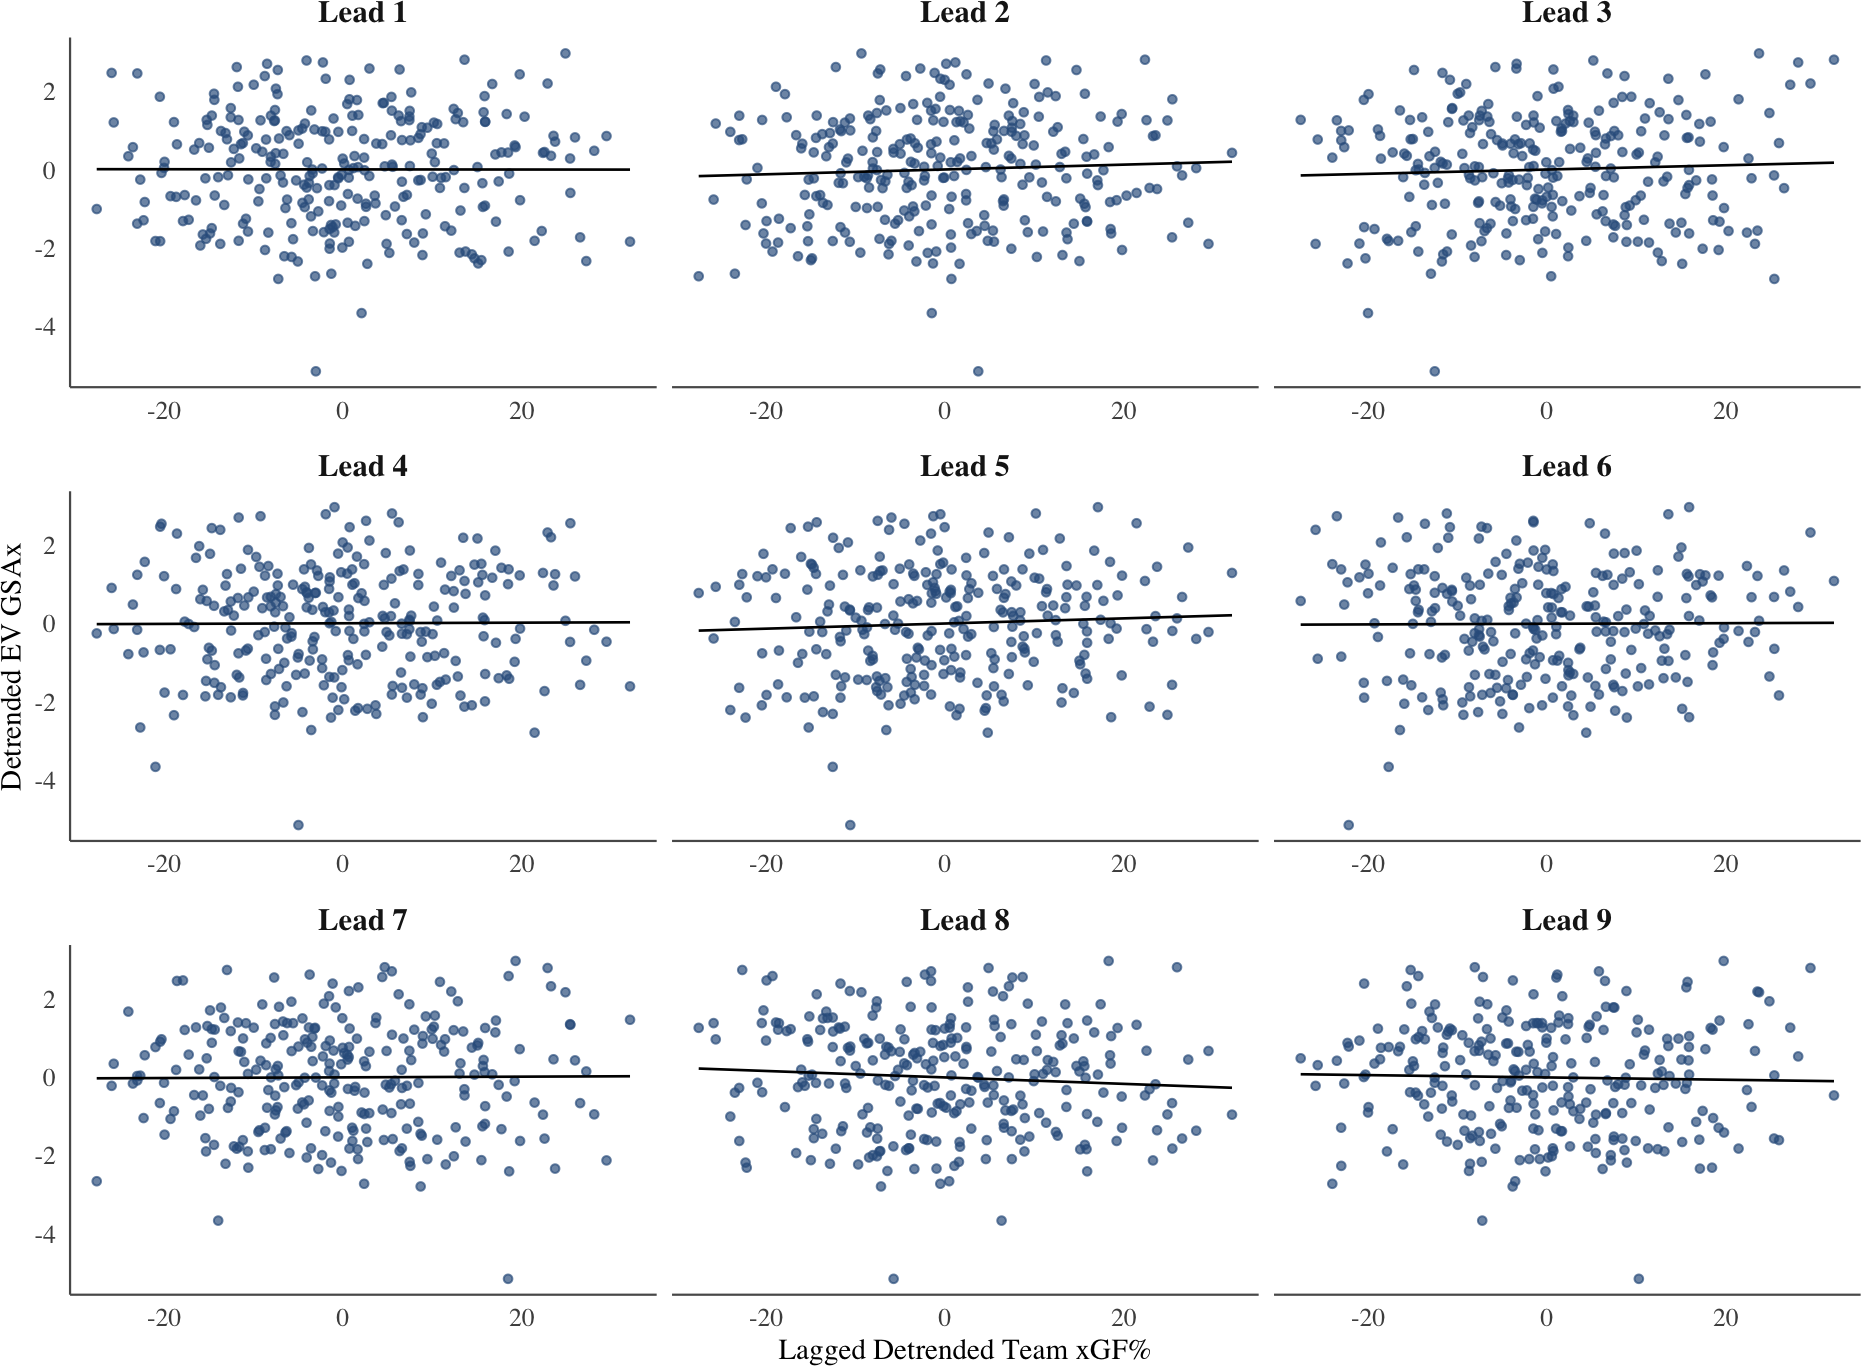
\includegraphics[width=\linewidth]{Paper_files/figure-latex/scatter-blackwood-xgf-1} 

}

\caption{Blackwood detrended GSAx against lagged detrended team xGF\%.}\label{fig:scatter-blackwood-xgf}
\end{figure}

Figure \ref{fig:scatter-blackwood-xgf} gives the same lead-by-lead view for Blackwood's detrended team xGF\%. These panels are also scattered, which supports the main-paper conclusion that recent team context is not a strong direct predictor of Blackwood's current transformed detrended GSAx.

\begin{figure}[H]

{\centering 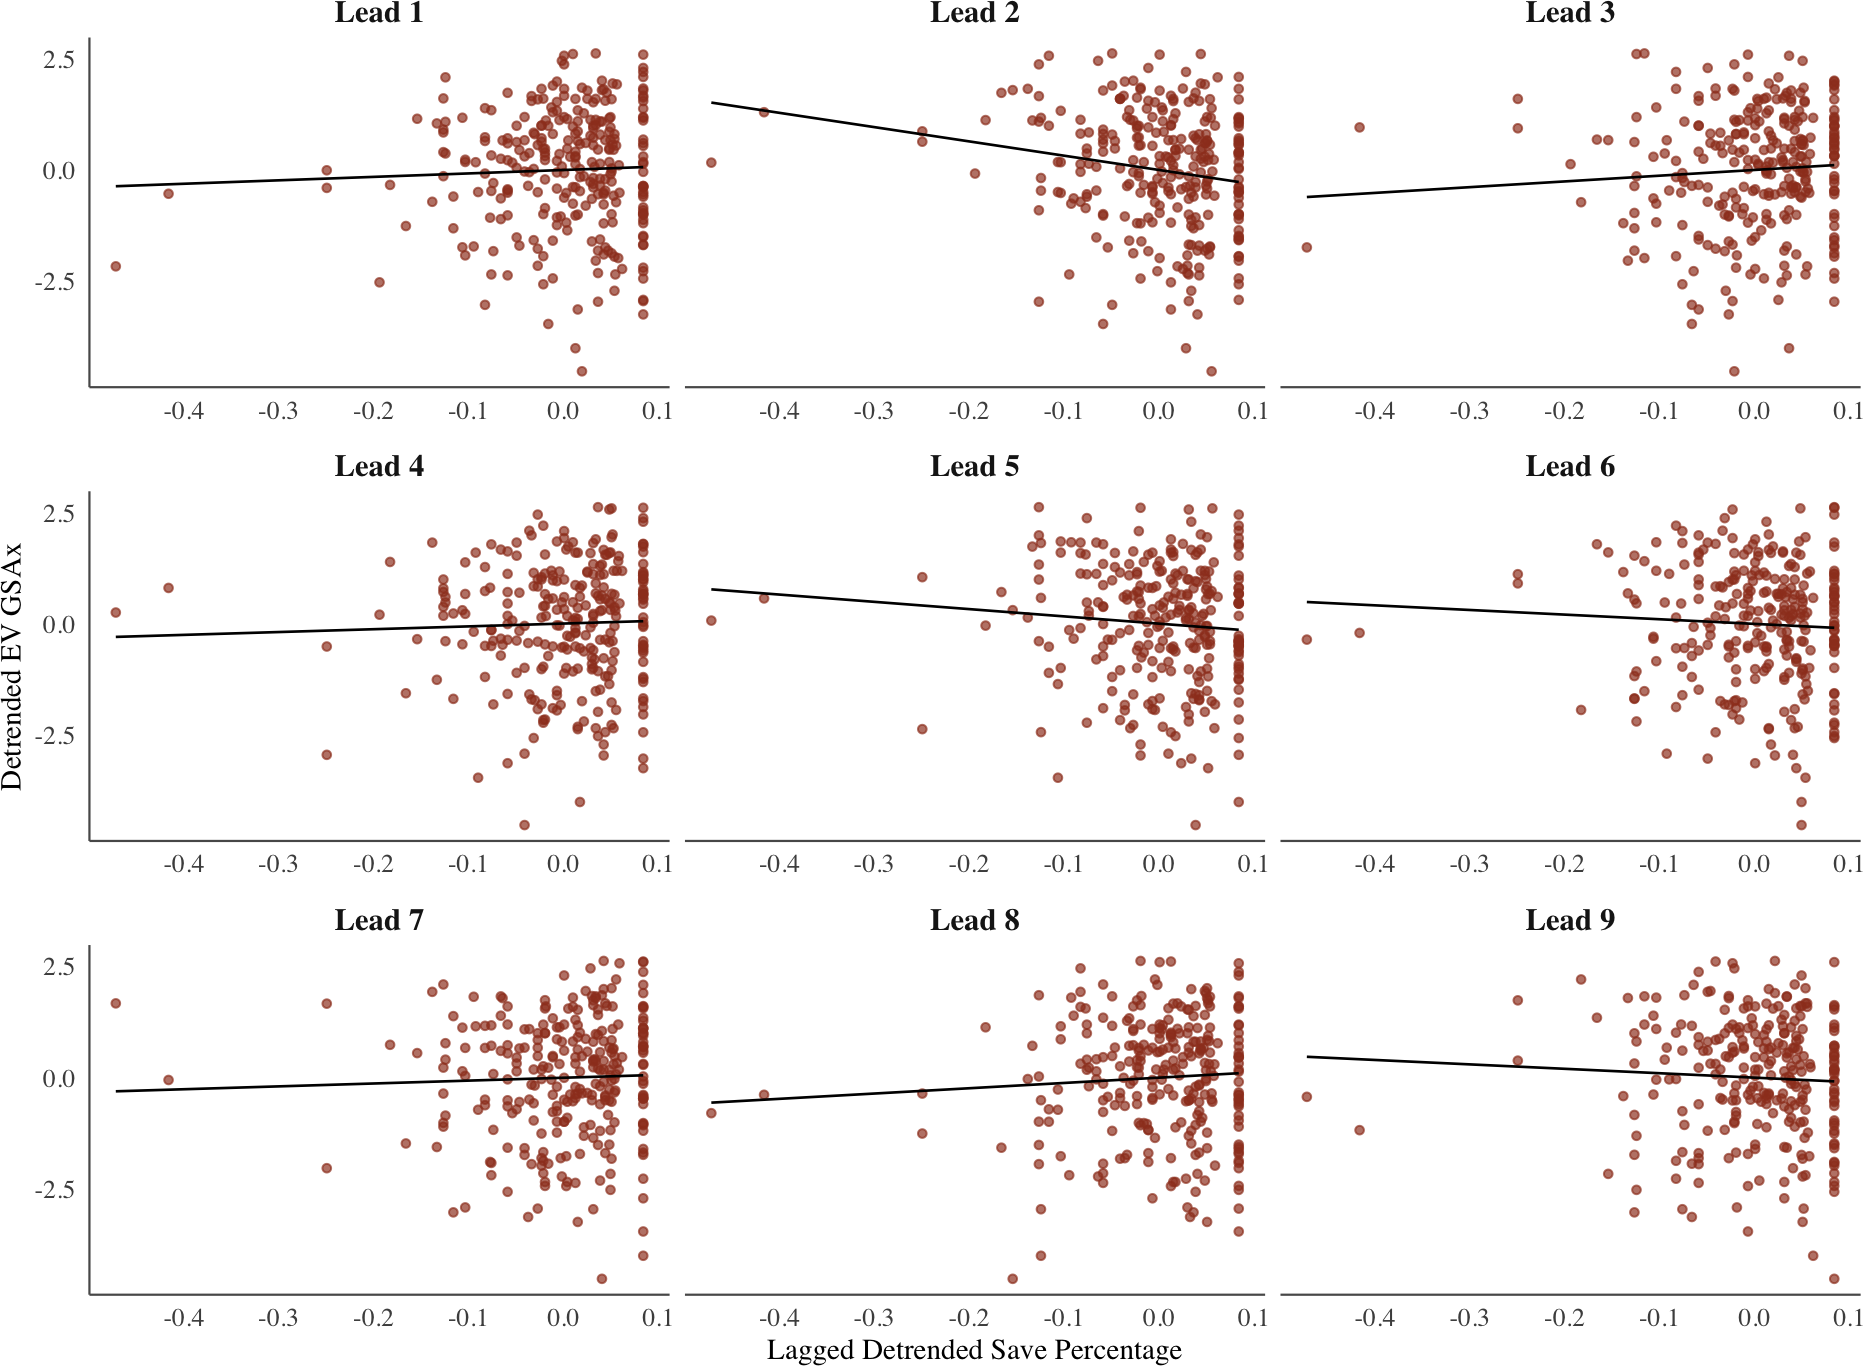
\includegraphics[width=\linewidth]{Paper_files/figure-latex/scatter-shesterkin-sv-1} 

}

\caption{Shesterkin detrended GSAx against lagged detrended save percentage.}\label{fig:scatter-shesterkin-sv}
\end{figure}

Figure \ref{fig:scatter-shesterkin-sv} shows Shesterkin's detrended GSAx against lagged detrended save percentage. The relationship is still noisy, but the shorter-lead panels, especially near the selected two-game lead, show the clearest visible pattern among the scatterplots.

\begin{figure}[H]

{\centering 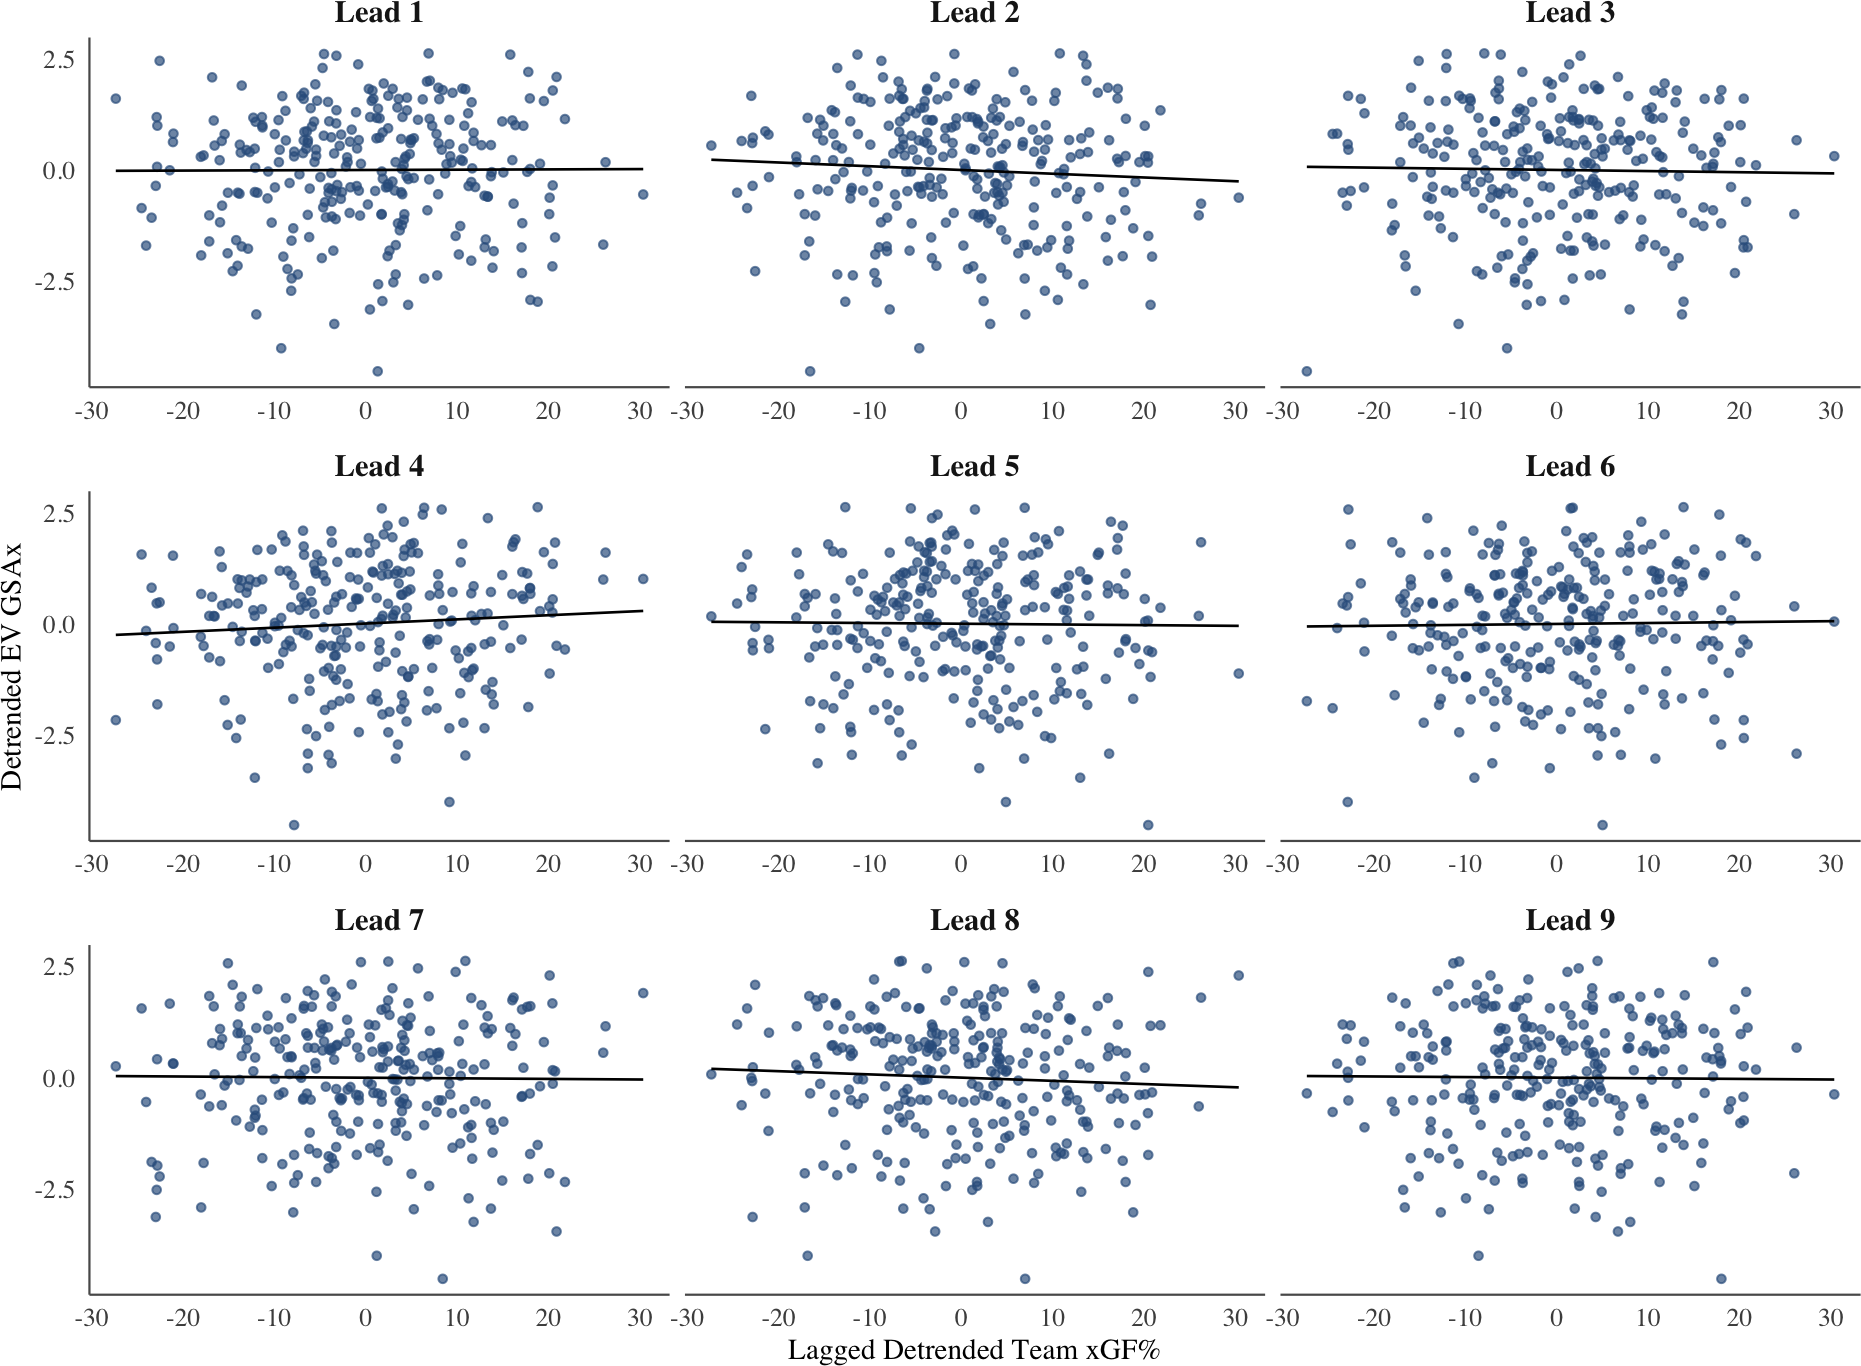
\includegraphics[width=\linewidth]{Paper_files/figure-latex/scatter-shesterkin-xgf-1} 

}

\caption{Shesterkin detrended GSAx against lagged detrended team xGF\%.}\label{fig:scatter-shesterkin-xgf}
\end{figure}

Figure \ref{fig:scatter-shesterkin-xgf} shows Shesterkin's detrended GSAx against lagged detrended team xGF\%. The panels remain much more scattered than the save-percentage panels, so any team-context effect is weak in this direct lagged-regression setup.

\begin{table}[H]
\centering
\caption{\label{tab:transform-table}Transformation review for aligned detrended GSAx response.}
\centering
\resizebox{\ifdim\width>\linewidth\linewidth\else\width\fi}{!}{
\fontsize{6.8}{8.8}\selectfont
\begin{tabular}[t]{lcrrrrr}
\toprule
Goalie & Series & Shift & Lambda & Raw Ratio & Log Ratio & Box-Cox Ratio\\
\midrule
Blackwood & $\tilde{G}_t$ & 6.1500 & 1.6711 & 0.9276 & 0.7313 & 0.9781\\
Shesterkin & $\tilde{G}_t$ & 5.5209 & 1.9999 & 1.4789 & 1.9401 & 1.3248\\
\bottomrule
\end{tabular}}
\end{table}

Table \ref{tab:transform-table} documents why the response was transformed before the final time-series regressions. The predictors remain in detrended original units because the transformation review did not justify making the whole model less interpretable.

\subsection{Appendix B: Fitted Equations and Coefficients}\label{appendix-b-fitted-equations-and-coefficients}

For Blackwood, the transformed regression is
\[
Y^{(B)}_t = 12.17295 - 5.52336 \tilde{S}_{t-4} - 0.03208 \tilde{X}_{t-8} + W_t.
\]
For Shesterkin, the transformed regression is
\[
Y^{(S)}_t = 15.70090 - 17.00071 \tilde{S}_{t-2} + 0.05423 \tilde{X}_{t-4} + W_t.
\]

The original-scale fitted equations are shown in the main Results section so the final model can be read before the residual diagnostics and forecast.

\begin{table}[H]
\centering
\caption{\label{tab:coef-tables}Time-series regression coefficient estimates.}
\centering
\resizebox{\ifdim\width>\linewidth\linewidth\else\width\fi}{!}{
\fontsize{6.8}{8.8}\selectfont
\begin{tabular}[t]{lcrrrc}
\toprule
Goalie & Term & Estimate & Std. Error & t Value & P-value\\
\midrule
Blackwood & Intercept & 12.17295 & 0.27638 & 44.0449 & <0.0001\\
Blackwood & $\tilde{S}_{t-4}$ & -5.52336 & 3.51831 & -1.5699 & 0.1176\\
Blackwood & $\tilde{X}_{t-8}$ & -0.03208 & 0.02223 & -1.4432 & 0.1501\\
Shesterkin & Intercept & 15.70090 & 0.41745 & 37.6119 & <0.0001\\
Shesterkin & $\tilde{S}_{t-2}$ & -17.00071 & 5.61708 & -3.0266 & 0.0027\\
Shesterkin & $\tilde{X}_{t-4}$ & 0.05423 & 0.03756 & 1.4437 & 0.1500\\
\bottomrule
\end{tabular}}
\end{table}

Table \ref{tab:coef-tables} reports the coefficient-level evidence for the transformed lagged regressions. Blackwood's individual lag coefficients are weak, matching the main-text conclusion that the two selected lagged predictors do not jointly explain much of his current transformed detrended GSAx. Shesterkin's lagged save-percentage coefficient is more informative statistically, but the model still explains only a small share of the total game-to-game variation.

\begin{table}[H]
\centering
\caption{\label{tab:regression-summary-table}Transformed lagged-regression fit criteria.}
\centering
\resizebox{\ifdim\width>\linewidth\linewidth\else\width\fi}{!}{
\fontsize{6.4}{8.4}\selectfont
\begin{tabular}[t]{lcrrrrrrrr}
\toprule
Goalie & Predictors & Lambda & Shift & \# Parameters & $R_a^2$ & $p_F$ & AIC & AICc & BIC\\
\midrule
Blackwood & $\tilde{S}_{t-4},\tilde{X}_{t-8}$ & 1.6711 & 6.1500 & 3 & 0.0083 & 0.1182 & 5.9078 & 4.0704 & 5.9601\\
Shesterkin & $\tilde{S}_{t-2},\tilde{X}_{t-4}$ & 1.9999 & 5.5209 & 3 & 0.0324 & 0.0038 & 6.7467 & 4.9094 & 6.7985\\
\bottomrule
\end{tabular}}
\end{table}

Table \ref{tab:regression-summary-table} gives the regression fit criteria in the same compact form used throughout the semester: number of parameters, adjusted \(R^2\), F-test p-value, and likelihood-based criteria. The key contrast is that Shesterkin has a statistically significant overall F-test while Blackwood does not, but both adjusted \(R^2\) values remain small enough that the results should be interpreted cautiously.

\begin{table}[H]
\centering
\caption{\label{tab:forecast-eval-table}Transformed lagged-regression forecast evaluation under the aligned Colorado split.}
\centering
\resizebox{\ifdim\width>\linewidth\linewidth\else\width\fi}{!}{
\fontsize{6.8}{8.8}\selectfont
\begin{tabular}[t]{lrrrrr}
\toprule
Goalie & ME & MPE & MSE & MAE & MAPE\\
\midrule
Blackwood & 1.6578 & 1.7050 & 20.4186 & 3.6195 & 29.2076\\
Shesterkin & -0.3084 & -76.7164 & 56.5631 & 6.1096 & 101.2303\\
\bottomrule
\end{tabular}}
\end{table}

Table \ref{tab:forecast-eval-table} reports the five forecast evaluation metrics. The split is Blackwood's first Colorado game, applied to both goalies by matched career game number, and the errors are measured on the transformed lagged-regression response scale. Blackwood has smaller MSE and MAE than Shesterkin under this split, but both holdout summaries still show large errors relative to the small adjusted \(R^2\) values in Table \ref{tab:regression-summary-table}. Therefore, the forecast evaluation supports the same practical conclusion as the fit table: the lagged predictors produce, at best, modest short-run forecasting value.

\subsection{Appendix C: ARMA, ARIMA, and Auto-ARIMA Details}\label{appendix-c-arma-arima-and-auto-arima-details}

\begin{figure}[H]

{\centering 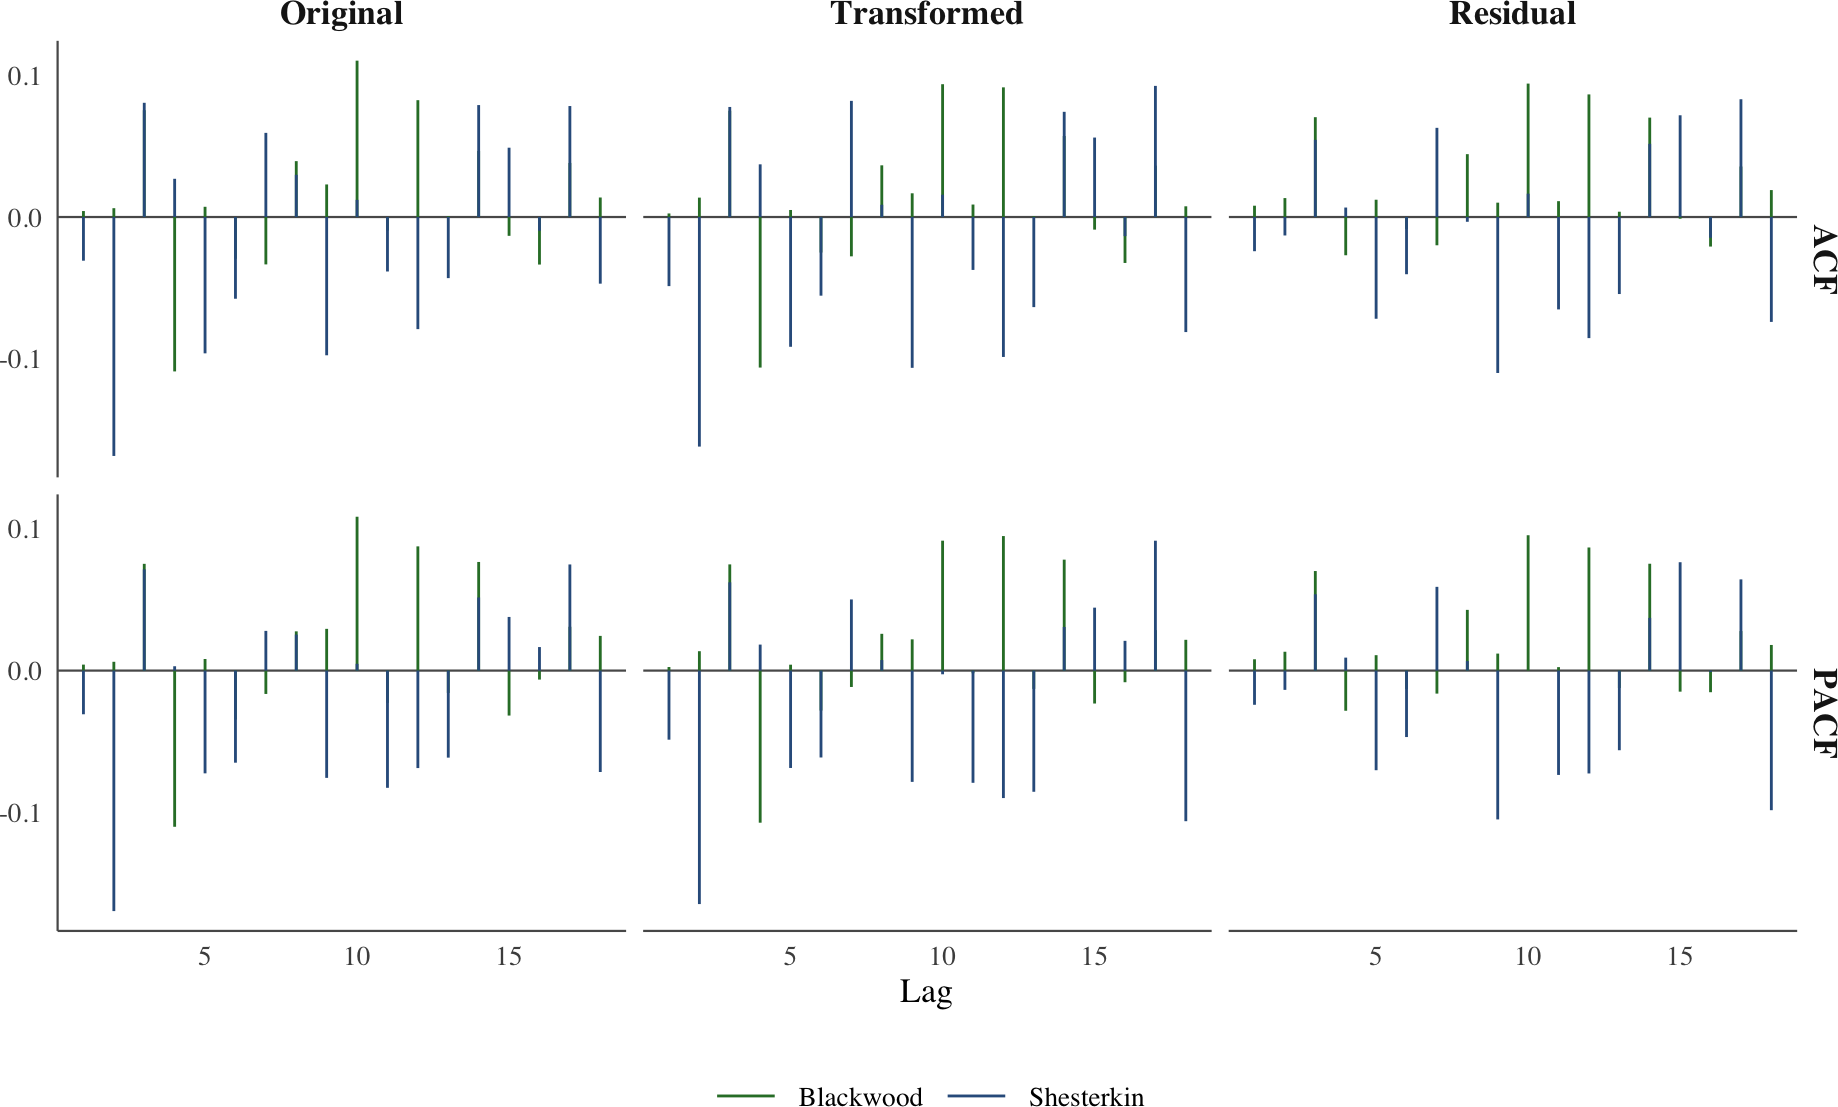
\includegraphics[width=\linewidth]{Paper_files/figure-latex/acf-pacf-comparison-1} 

}

\caption{ACF and PACF comparison for original response, transformed response, and final residuals.}\label{fig:acf-pacf-comparison}
\end{figure}

Figure \ref{fig:acf-pacf-comparison} compares the original response, transformed response, and final residuals. The residual panels are the important final check: after detrending, transformation, and lagged regression, the remaining ACF and PACF spikes are small and do not show a persistent dependence pattern.

\begin{table}[H]
\centering
\caption{\label{tab:arma-candidates-blackwood}Blackwood ARMA candidates for regression residuals.}
\centering
\resizebox{\ifdim\width>\linewidth\linewidth\else\width\fi}{!}{
\fontsize{6.8}{8.8}\selectfont
\begin{tabular}[t]{lrrrrrr}
\toprule
Model & p & d & q & \# Predictors & $\hat{\sigma}_W^2$ & AIC\\
\midrule
ARIMA(0,0,0) & 0 & 0 & 0 & 0 & 20.9264 & 1630.45\\
ARIMA(1,0,0) & 1 & 0 & 0 & 1 & 20.9250 & 1632.43\\
ARIMA(0,0,1) & 0 & 0 & 1 & 1 & 20.9251 & 1632.43\\
ARIMA(1,0,1) & 1 & 0 & 1 & 2 & 20.9251 & 1634.43\\
ARIMA(2,0,0) & 2 & 0 & 0 & 2 & 20.9213 & 1634.39\\
ARIMA(0,0,2) & 0 & 0 & 2 & 2 & 20.9216 & 1634.39\\
ARIMA(2,0,1) & 2 & 0 & 1 & 3 & 20.8340 & 1635.26\\
ARIMA(1,0,2) & 1 & 0 & 2 & 3 & 20.8514 & 1635.48\\
\bottomrule
\end{tabular}}
\end{table}

Table \ref{tab:arma-candidates-blackwood} shows the low-order ARMA comparison for Blackwood's transformed-regression residuals. ARIMA(0,0,0) has the lowest AIC, so the residual model is white noise rather than an additional AR or MA dependence model.

\begin{table}[H]
\centering
\caption{\label{tab:arma-candidates-shesterkin}Shesterkin ARMA candidates for regression residuals.}
\centering
\resizebox{\ifdim\width>\linewidth\linewidth\else\width\fi}{!}{
\fontsize{6.8}{8.8}\selectfont
\begin{tabular}[t]{lrrrrrr}
\toprule
Model & p & d & q & \# Predictors & $\hat{\sigma}_W^2$ & AIC\\
\midrule
ARIMA(0,0,0) & 0 & 0 & 0 & 0 & 48.4430 & 1889.83\\
ARIMA(1,0,0) & 1 & 0 & 0 & 1 & 48.4148 & 1891.67\\
ARIMA(0,0,1) & 0 & 0 & 1 & 1 & 48.4141 & 1891.67\\
ARIMA(1,0,1) & 1 & 0 & 1 & 2 & 48.4134 & 1893.66\\
ARIMA(2,0,0) & 2 & 0 & 0 & 2 & 48.4057 & 1893.62\\
ARIMA(0,0,2) & 0 & 0 & 2 & 2 & 48.4088 & 1893.63\\
ARIMA(2,0,1) & 2 & 0 & 1 & 3 & 48.3750 & 1895.44\\
ARIMA(1,0,2) & 1 & 0 & 2 & 3 & 48.3812 & 1895.48\\
\bottomrule
\end{tabular}}
\end{table}

Table \ref{tab:arma-candidates-shesterkin} gives the same ARMA comparison for Shesterkin. The selected residual model is again ARIMA(0,0,0), which agrees with the residual ACF in Figure \ref{fig:residual-diagnostics}: after the transformed regression, there is no useful remaining serial dependence to model.

\begin{table}[H]
\centering
\caption{\label{tab:arima-candidate-table}First-differenced ARIMA candidates for regression residuals.}
\centering
\resizebox{\ifdim\width>\linewidth\linewidth\else\width\fi}{!}{
\fontsize{6.5}{8.5}\selectfont
\begin{tabular}[t]{llrrrrrr}
\toprule
Goalie & Model & p & d & q & \# Predictors & $\hat{\sigma}_W^2$ & AIC\\
\midrule
Blackwood & ARIMA(0,1,0) & 0 & 1 & 0 & 0 & 41.5682 & 1814.00\\
Blackwood & ARIMA(1,1,0) & 1 & 1 & 0 & 1 & 31.0311 & 1735.60\\
Blackwood & ARIMA(0,1,1) & 0 & 1 & 1 & 1 & 21.1021 & 1632.00\\
Blackwood & ARIMA(1,1,1) & 1 & 1 & 1 & 2 & 21.1021 & 1633.99\\
Blackwood & ARIMA(2,1,0) & 2 & 1 & 0 & 2 & 26.7430 & 1696.86\\
Blackwood & ARIMA(0,1,2) & 0 & 1 & 2 & 2 & 21.1021 & 1633.99\\
Blackwood & ARIMA(2,1,1) & 2 & 1 & 1 & 3 & 21.1023 & 1635.99\\
Blackwood & ARIMA(1,1,2) & 1 & 1 & 2 & 3 & 21.0921 & 1635.89\\
Shesterkin & ARIMA(0,1,0) & 0 & 1 & 0 & 0 & 99.4429 & 2084.49\\
Shesterkin & ARIMA(1,1,0) & 1 & 1 & 0 & 1 & 73.9446 & 2003.83\\
Shesterkin & ARIMA(0,1,1) & 0 & 1 & 1 & 1 & 48.6161 & 1891.75\\
Shesterkin & ARIMA(1,1,1) & 1 & 1 & 1 & 2 & 48.5884 & 1893.63\\
Shesterkin & ARIMA(2,1,0) & 2 & 1 & 0 & 2 & 63.2621 & 1962.45\\
Shesterkin & ARIMA(0,1,2) & 0 & 1 & 2 & 2 & 48.5879 & 1893.63\\
Shesterkin & ARIMA(2,1,1) & 2 & 1 & 1 & 3 & 48.5799 & 1895.60\\
Shesterkin & ARIMA(1,1,2) & 1 & 1 & 2 & 3 & 48.5869 & 1895.63\\
\bottomrule
\end{tabular}}
\end{table}

Table \ref{tab:arima-candidate-table} checks whether first differencing the regression residuals improves the residual model. The best first-differenced candidates have higher AIC than the manual ARMA(0,0) choices, so the differenced ARIMA step does not change the final modeling decision.

\begin{table}[H]
\centering
\caption{\label{tab:auto-table}auto.arima comparison on raw GSAx with raw save percentage and team xGF\% as xreg.}
\centering
\resizebox{\ifdim\width>\linewidth\linewidth\else\width\fi}{!}{
\fontsize{6.8}{8.8}\selectfont
\begin{tabular}[t]{lccrrr}
\toprule
Goalie & Xreg & Model & $\hat{\sigma}^2$ & AIC & BIC\\
\midrule
Blackwood & $S_t,X_t$ & ARIMA(0,1,1) & 0.6856 & 706.58 & 721.17\\
Shesterkin & $S_t,X_t$ & ARIMA(0,1,1) & 0.4666 & 598.03 & 612.62\\
\bottomrule
\end{tabular}}
\end{table}

Table \ref{tab:auto-table} gives the automated comparison requested in the assignment. The selected model is ARIMA(0,1,1) for both goalies, which is more complex than the final manual residual model but still short-memory: after one difference, the remaining dependence is captured by one moving-average term. This supports the main paper's comparison because the automated route finds some local dependence, while the final lagged-regression route shows that the dependence does not translate into strong explanatory power for game-level GSAx.

\end{document}
